\chapter{The Game}
\section{Basic Gameplay} \label{basic-gameplay}
The objective of the game is to score the most points by capturing the opponents' flags while keeping your own safe.
A game is broken down in the following way:
\begin{enumerate}
    \item A game consists of three acts, called Thirds.
    These work similar to half-times in most sports.
    % TODO: Find a way to possibly automate this
    \item The game starts with rock-paper-scissors, dice roll, or other means to determine who goes first.
    % TODO: introduce a play-book mechanic
    \item Each player starts a Third by positioning their units on their side of the board.
    Positioning units goes clockwise around the board, starting with the first player.
    \item Once a player is done positioning their units, they may not try and reposition them in response to the placement of the other teams’ units.
    \item A character can do one of five things on its turn:
    \begin{enumerate}
        \item Do nothing.
        \item Move a number of hexes less than or equal to their move score.
        \item Attack an opponent (see Section \ref{skill-checks}).
        \item Throw or Pass a flag (see Section \ref{flag-interaction})
        \item A special action, which may require Source (see Section \ref{energy}).
    \end{enumerate}
    \item A flag is picked up automatically upon touching, unless it’s either thrown at you or rolling towards you (see Section \ref{flag-interaction}).
    \item Bringing a flag does not automatically end a Third unless either
    \begin{enumerate}
        \item All three flags are in the same capture zone
        \item The Heavy is captured
    \end{enumerate}
\end{enumerate}

\section{The Team} \label{the-team}
Each team consists of 7 characters, each with five stats:

\begin{description}
    \item[Strength (Str)] Strength determines your attack power, and your ability to keep your balance if your attack fails.
    \item[Dexterity (Dex)] Dexterity determines how well you throw and catch the flag.
    \item[Throw (Thr)] Throw is your actual throwing distance. It is $Dex/2$ by default.
    \item[Agility (Agi)] Agility determines how well you dodge and run.
    \item[Move (Mov)] Move is the actual running distance. It is $Agi / 2$ by default.
\end{description}
Each character can also have zero or more special abilities. 
These abilities are additional modifiers that can change up how characters act. 
An example ability could be giving an attacking opponent a smaller chance of succeeding, or being able to leap great distances.

%\section{Skill Rolls}\label{skill-rolls}
Skill rolls are used to determine the outcome of certain actions, and each skill has an associated skill roll that needs to be performed in special occasions.

To perform a skill roll, a player rolls 3d6 against a character's given skill.
If the player rolls the exact value or below, it's a success; if the player rolls above it's a fail.

If a player rolls a 3 (\epsdice{1}\epsdice{1}\epsdice{1}), it is called a ``critical success''; similarly if a player rolls 18 (\epsdice{6}\epsdice{6}\epsdice{6}), it is called a ``critical failure''.
These special outcomes have special connotation in certain contexts.

\example{If your character's Dexterity is 12 and you roll 10 with 3d6, you succeed that roll.}

\note{Whenever this manual refers to ``rolling against'' a certain skill, we're talking about a skill roll.}

\subsection{Strength}
Strength rolls are required whenever you roll $+$ or $-$ on an attack (see Section \ref{attacking}).
The outcome of a strength roll determines whether you ultimately succeed or fail your roll.

\paragraph{Critical Success} If you successfully roll a 3 on an attack, you not only knock out an opponent's character, you get to take it off the field until the next third of the match.

\paragraph{Critical Failure} If you roll an 18 on an attack your own character gets knocked out until the next third.
\subsection{Dexterity}
Dexterity rolls are required whenever you try to throw, pass, catch, or intercept a flag.
A success means it goes as planned, a fail means it doesn't (see Section \ref{flag-interaction}).

\paragraph{Critical Success} A critical success means the throw is executed exactly the way you want it to.
You don't have to roll to catch, and the enemy doesn't get to intercept.

\subsection{Agility}
Agility rolls are required whenever you want to invoke the Sprint action (see Section \ref{special-action}).
A success means your character gets to move the extra distance, a fail means they fall on their face.
\section{Actions \& Skill Checks}\label{skill-checks}
During the game, many physical altercations will need to be modelled.
To achieve this, we use \textit{Skill Checks}; wherein you directly compare the physical characteristics---or \textit{skills}---of two or more players.

In checking skills, you will also have to roll for your player's \fate{}.
This is done with a \textit{Fate Die}.
The outcome of this die could either add or subtracts 1 from the player's skill.

A player has three principle actions they can perform, which require skill checks: \textit{attacking}, \textit{tackling}, and \textit{dodging}.

\subsection{Harming (Fight vs. Flight)}
When a player attempts to harm another player, you compare the attacking player's \fight{} skill against the defending player's \flight{} skill, taking the relevant \fate{} rolls into account.

\paragraph{Success}
The opposing player gets knocked down, remaining in the hex where they stood.
\paragraph{Failure}
The defending coach moves the attacking player into an adjacent hex.
\paragraph{Stalemate}
Nothing happens.
The players remain in their respective hexes.

\subsection{Shove (Fight vs. Fight)}
When a player attempts to shove another player, you compare their \fight{} skills, taking the relevant \fate{} rolls into account.

\paragraph{Success} 
The opposing player gets knocked down. 
The attacking coach gets to move the downed player to an adjacent hex.
The attacking player moves into the previously occupied hex.

\begin{note}
In the event that multiple players are in a dogpile (see \secref{dogpiling}), all the participating players are elegible to move into the previously occupied hexes as the victor sees fit.
\end{note}
\paragraph{Failure}
The attacking player gets knocked down where they stand.
\paragraph{Stalemate}
Nothing happens.
The players remain in their respective hexes.

\subsection{Dodging (Flight vs. Fight)}
If your player wishes to pass through an opposing player's reach (see \secref{moving}), compare your player's \flight{} skill against their \fight{} skill, adjusted for \fate{}.

\paragraph{Success}
Your player remains unaffected and may continue moving.
\paragraph{Failure}
Your player gets knocked down where they entered the defender's reach.
\paragraph{Stalemate}
The player remains where they would have exited the defender's reach, and get to remain standing.

\subsection{Snatching (Flight vs Flight)}
\paragraph{Success}
The player that was previously holding the flag or ball is knocked down.
Your player now holds the flag or ball.
\paragraph{Failure}
Your player is knocked down.
\paragraph{Stalemate}
Both the attacking and defending players are knocked down.
The flag or ball is scattered from the player who was originally holding it.
In case of a hit, scatter again, or use the arrow on the hit icon if one is present.

\begin{note}
In a dogpiling situation (see \secref{dogpiling}), only the attacking and defending players are knocked down, not any of the helpers or harrassers.
\end{note}

\subsection{Holding the Flag}
Holding the flag increases the radius of a player's reach by one hex.
It also prevents the player from being able to initiate shoves.

In lieu of a traditional pass, your player may attempt to throw the flag at an opposing player as a ranged attack.
You roll an \textit{Attack} as normal.
If it fails, treat as a failed \throw{} instead (See \secref{flag-interaction}).

\subsection{Accounting for Multiple Players (Dogpiling)}\label{dogpiling}
In the event of mutually overlapping player reaches during an attack, the coaches may opt to have multiple players join in the dogpile.
Players are only able to join the dogpile if an enemy in their reach is already in the dogpile.
When doing this, you combine the relevant skill of all involved players and roll their combined total number of fate dice. 
See \secref{combat-step-by-step} for a breakdown.

\subsection{Combat Step-by-Step}\label{combat-step-by-step}
Here is a simplified breakdown of combat.
\begin{enumerate}
    \item Attacker declares type of attack and target
    \item Attacker declares helpers
    \item Defender declares helpers
    \item Harrier declares harrassers
    \item Combat resolves en masse
    \item Depending on outcome, the coaches may move players accordingly
    \item If successful, attacker's helpers are free to act.
\end{enumerate}

\begin{note}
Here, \textit{Harrier} refers to the coach that isn't either the attacker or defender. 
The harrier can choose to act on either side of the conflict, or both of them at once as they see fit.
\end{note}

% | Actor | Reactor | Outcome |
% |-------+---------+---------|
% | Fgt   | Fgt     | Grapple |
% | Fgt   | Flt     | Dodge   |
% | Flt   | Fgt     | Block   |
\section{Moving} \label{moving}
A character's movement is defined by their Agility score.
By default, a character can move $Agi / 2$ number of hexes (rounded down).
So if the character has an agility of 13, they can move at most 6 hexes in a single turn.
That this can change if a character's special ability says otherwise.

\paragraph{Note} You \textit{\textbf{cannot}} go back to a character you have already moved.

\subsection{Tackle Zones \& Opportunity Attacks}
Every character has a tackle zone around them (see Figure~\ref{fig:tackle-zone-1}).
The tackle zone is made up of every hex immediately around a character.

If an opponent \textit{leaves} a hex within the tackle zone of your character, they must first roll against their agility score to see if they successfully dodge your attack.
If they fail, you get to attack them as normal (see \textit{Attacking} in Section \ref{attacking}).
If they succeed, they get to move as usual.

\paragraph{Note} Tackle zones can also overlap (see figure \ref{fig:tackle-zone-2}).
If your character tries to move out of an overlapping tackle zone, only roll for the one you're actually leaving.
If you're leaving both at once, you must escape the one with the highest Agility first.
Failing one fails them both.

\begin{figure}
    \centering
    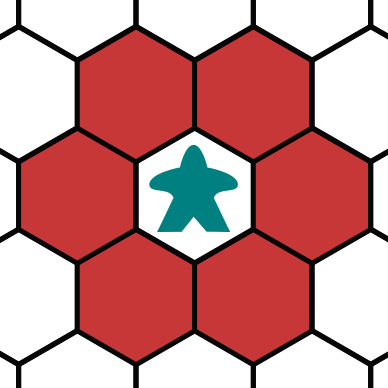
\includegraphics{graphics/tackle-zones-1.png}
    \caption{The tackle zone around a character.}
    \label{fig:tackle-zone-1}
\end{figure}

\begin{figure}
    \centering
    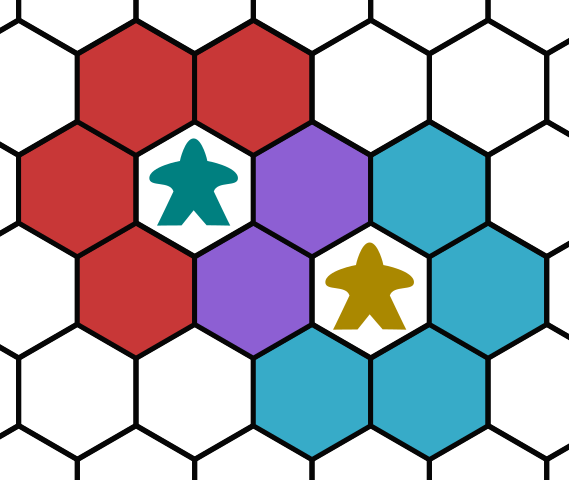
\includegraphics{graphics/tackle-zones-2.png}
    \caption{The overlapping tackle zones between two characters.}
    \label{fig:tackle-zone-2}
\end{figure}
%\section{Attacking} \label{attacking}
Attacking involves first rolling a Fate Die\footnote{This is also commonly called ``rolling for fate'', since a) it's a fate die, and b) it determines the fate of the attacker} to see if your attack succeeds.
The die has three different outcomes: $+$, $-$, and blank; depending on the outcome you either succeed, fail, or push respectively.
For every person helping you, you get to roll an additional attack die (see Section~\ref{sec:multidice}).

\subsection{Succeeding an Attack (Rolling $+$)}
On a successful attack, you roll against your Strength score to see if you successfully knock your opponent into the ground.
Doing so successfully, causes them to get pushed one hex and knocked over.
You then have the option of moving into the hex they just occupied.

\paragraph{Note} The effect of the roll \textit{modifies} how your roll is performed.
For example, if your character has a base Strength of 10, and you roll $++$, then you need to roll 11 or less to succeed, since in this case $Str+1=11$.

Additionally, failing your Strength check results in the attack just becoming a push (see Pushing).
Succeeding your Strength check results in the opponent to be pushed into an adjacent hex and then knocked down, leaving them out until their next turn.

\subsection{Failing an Attack (Rolling $-$)}
When you fail an attack, you must roll against Strength to see if you yourself fumble and fall on your face.

If you fail your fail roll, you will fall on your face and be knocked out for the rest of the turn.
Succeeding the fail roll means nothing happens.

\subsection{Pushing (Rolling a Blank)}
Whenever you roll a blank, your attack does not get a chance to knock someone out, you merely push them.
When you push an opponent, you move them into one of \textit{their} adjacent hexes.
After doing so, you have the option of moving into the space they just occupied.

\subsection{Rolling Multiple Dice}\label{sec:multidice} If the result of rolling multiple fate dice contains both $+$'s and $-$'s, you may choose whether it's a success ($+$) or a failure ($-$).
Then you add together the values of the remaining dice, to determine the advantage/disadvantage gained from the roll.

\begin{example}
    Alice chooses to use her Bruiser to attack Bob's piece with two of her pieces helping in the attack.
\end{example}
She rolls 3 fate dice and rolls $+, -, 0$.
She decides to take the risk, and has it be a success with a $-1$ disadvantage, which sets her Bruiser's attack to 11, 1 less than the default of 12.

\subsection{Getting Knocked Out}\label{sec:knockout}
If your character is knocked to the ground, they're out until your next turn.
A knocked out character has no tackle zone, and cannot attack.

On your next turn you have the option of having the character get back up.
Doing so counts as moving two hexes, meaning if you do not use your character after getting it back up, it counts as a wasted move.

\begin{note} 
Because of the movement penalty for getting back up, attacking with a character that's just gotten up requires a \textit{Tackle} (see Section~\ref{energy}).
\end{note}
\section{Specials \& Source}\label{energy}
\subsection{Specials}
In addition to the basic moves, each character has zero or more special abilities, tied to the character type. 
These special abilities can be activated when the right criteria are met, and can have a profound impact on the gameplay.

Some special abilities have an associated Source cost that must be paid in order to activate the special ability.

\begin{figure}
    \centering
    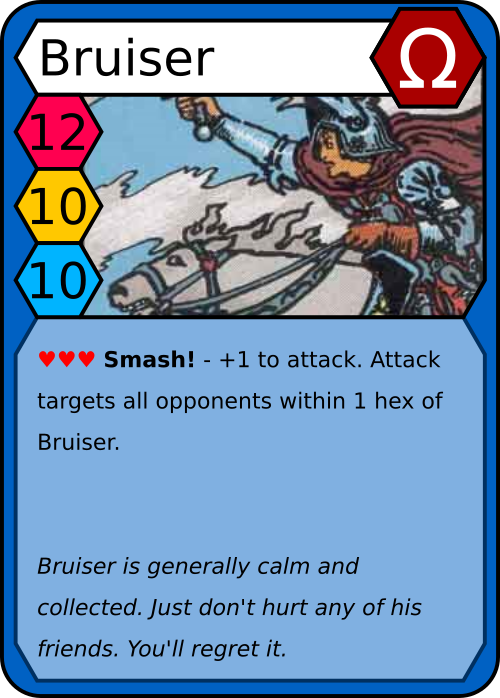
\includegraphics{graphics/bruiser-red.png}
    \caption{Special ability with associated Source cost.}
    \label{fig:ability-example}
\end{figure}

Figure~\ref{fig:ability-example} shows a character with a special ability called \textit{Smash!}.
Smash! requires three Hearts Source to be activated and provides the written bonus.

In addition to the special abilities written on each card, each team also has one or more special ability that applies universally to all characters on a team.

\note Any number of abilities can be activated per turn, as long as there's enough Source to do so.
\subsection{Source}
Source is a special resource available to \textit{all} players in the game, which facilitates the activation of special abilities. Each player may activate any number of special abilities on their own turn, as long as there's enough Source to do so.

\subsubsection{Source Types}
There are four different types of \textit{Source}, \textit{Hearts}, \textit{Spades}, \textit{Clubs}, \textit{Diamonds}\footnote{These are just for play-testing, and will be changed in the final version of the game}, as well as a fifth special type, \textit{Stars}.
Stars act as a wild-card and can consume any colour of Source.

\begin{figure}
    \centering
    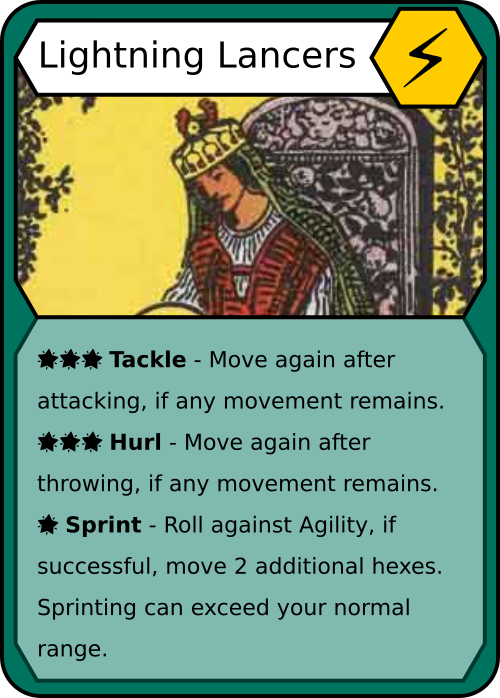
\includegraphics{graphics/yellow-team.png}
    \caption{Team card with wild-card Source abilities.}
    \label{fig:ability-example-2}
\end{figure}

Figure~\ref{fig:ability-example-2} shows a card that uses Stars as the ability cost.
Stars are considered colourless.
\subsubsection{Source Pool}
The Source Pool is the set of common Source cards available to all players, and is indicated by four or more face-up Source cards on the table.
To activate an ability discard the required number of Source cards of a given colour to consume them, then follow the ability's instructions as printed on the card.
Replenish the Source pool by drawing new cards, equal to the number of spent cards at the beginning of the next player's turn.

The number of Source cards increases every Third.
\subsubsection{Source Pool Size}
\begin{description}
    \item[1st Third] The Source pool contains 4 cards
    \item[2nd Third] The Source pool contains 6 cards
    \item[3rd Third] The Source pool contains 8 cards.
\end{description}
\section{Flag Interaction} \label{flag-interaction}
This section codifies the rules for how flags are interacted with, as well as what the two different flag types can and cannot do.

Flags are picked up automatically when they're touched by a player's character, this ends that character's turn (unless otherwise specified).
The exceptions being when it's thrown at someone, or rolls towards someone.

\subsection{The Spear}
The spear is the flag present at each of the teams' capture zones.
The spear can be thrown to other characters, and needs to be caught, the throw increases in difficulty as the distance it needs to be thrown increases.
A failed catch means the catcher is knocked out until the player's next turn.

\begin{table}[!ht]
    \centering
\begin{tabular}{r|l}
    \textbf{Point Value} & 1 \\
    \textbf{Movement Penalty} & $None$ \\
    \textbf{Can be Thrown?} & Yes \\
    \textbf{Special Note} & Knocks people out if they fail to catch it \\
\end{tabular} 
    \caption{Spear Stats}
    \label{tab:spear}
\end{table}
The thrown Spear can be intercepted by an opponent's character.
To do this, the opponent must roll against their character's Dexterity to see if they successfully intercept the thrown flag.
If not, the flag simply continues flying towards its intended destination.

\subsection{The Heavy}
The Heavy is a special flag that resides in the middle of the board.
As its name implies it is heavy, and thus impedes movement, and cannot be thrown.
The Heavy cannot be thrown, only passed (see rules for passing below).
\begin{table}[!h]
    \centering
\begin{tabular}{r|l}
    \textbf{Point Value} & $\times 2$ \\
    \textbf{Movement Penalty} & $Move-2$ \\
    \textbf{Can be Thrown?} & No, but can be passed \\
    \textbf{Special Note} & Ends a Third the moment it’s captured.\\
\end{tabular}
    \caption{Heavy Stats}
    \label{tab:heavy}
\end{table}
The $\times 2$ point value applies to all the flags you have within your flag zone.
So if you have 0 flags, it becomes $0 \times 2 = 0$ points, but if you have all three flags, it becomes $3 \times 2 = 6$ points.
This incentivises both hunting down opponent flags, as well as keeping your own safe.
\subsection{Throwing}
To throw a flag at someone you must roll against your character’s dexterity.
A character can throw their $Dex / 2$ rounded down; meaning if your character has a dexterity level of 11, they can throw 5 hexes.
If you want to throw further than $Dex/2$ hexes, you can do so at a $-1$ penalty every 2 hexes you want to throw past the initial limit.
In other words, if your character can throw 5 hexes, and your target is 9 hexes away, then you roll against $Dex-2$ to succeed.

\paragraph{Note} Throwing can happen in any direction, not just along the six cardinals (see figure \ref{fig:line-throw}).

\begin{figure}
    \centering
    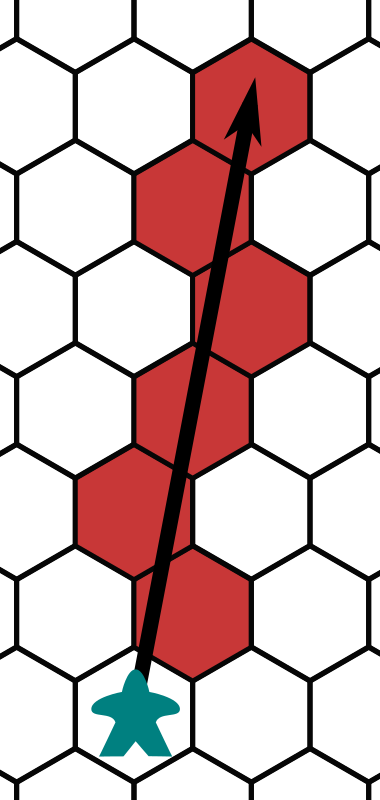
\includegraphics{graphics/throwing-cropped.png}
    \caption{A straight line approximated.}
    \label{fig:line-throw}
\end{figure}

\subsubsection{Failing a Throw}
If you fail a throw, roll a d6 and a fate die.
The d6 determines the distance it’s thrown, and the fate die determines how the throw diverges from the intended target.

Where the flag lands is determined in 2 steps:
\begin{enumerate}
    \item The Fate Die determines divergence
    \begin{enumerate}
        \item If you roll a +, the flag will fly towards the hex directly right of your intended target.
        \item If you roll a –, the flag will fly towards the hex directly left of your intended target.
        \item If you roll blank, the flag will not diverge from its intended target.
    \end{enumerate}
    \item The D6 is multiplied by 2 and determines distance.
    \begin{enumerate}
        \item If you roll a 1, the flag lands 2 hexes in front of the thrower.
        \item And if you roll 6, the flag lands 12 hexes away.
    \end{enumerate}
\end{enumerate}

\subsubsection{Chaining Throws}
Throws can also be chained.
If the character you're throwing the flag to hasn't acted yet, that character may throw the flag further.
This can be chained until you're out of usable characters.
\subsection{Passing}
Passing is the same as a throw, except the character you pass the flag to must be up to one hex away with nobody blocking the way.
Unlike throwing, passing cannot be intercepted.
\subsubsection{Failing a Pass}
If you fail a pass you roll a d6 and a fate die much like when you fail a throw.
However, because you’re passing a short distance, the d6 result is halved (rounded up), rather than doubled.
\subsection{Catching}
If you throw or pass the flag to someone, the flag must be caught.
Catching a flag requires rolling against Dex; a success means catching the flag, a fail means the recipient is knocked out (see Section~\ref{sec:knockout}), you then roll a d6 to determine in which hex around the recipient the flag lands.

\subsection{Getting Attacked}
If your character is attacked while holding a flag, the following happens:
\begin{description}
\item[Knocked Down] If your character is knocked down, the opponent gets to take the flag.
This does not apply to the Heavy, it is simply dropped instead, and you roll a d6 to see where it lands.
\item[Pushed] If your character is pushed, the opponent does not get the flag, it is merely pushed along.
\end{description}

\subsection{Dropping the Flag}
You can drop a flag as part of a regular move action.
You simply leave it where it is and continue moving.

\subsection{Out of Bounds}
If a player throws a flag out of bounds---out of the playing field---the previous player gets to place the flag on a hex of their choice in the middle zone.
\section{Scoring} \label{scoring}
Capturing a flag requires moving it into a capture zone and holding it there until the end of the Third.
Once a Third is over, all the flags in each capture zone are counted, and points are awarded to each player accordingly.
This means, if a player's flag was not stolen during the Third, or was stolen and returned, it counts as one point.
Thus, the least amount you can be rewarded is 0 points, and the most is 6 points.

\begin{note}
    Any flag can be stolen from capture zones by opposing players, including ones that do not belong to you!
\end{note}

\paragraph{Also Note} Holding a flag within a capture zone does not count it as being captured.
It \textit{must} be on the ground.
